% !TEX program = xelatex
% !TeX encoding = utf8
% !TeX spellcheck = pl-PL

%%%%%%%%%%%%%%%%%%%%%%%%%%%%%%%%%%%%%%%%%%%%%%%%%%%%%%%%%%%%%%%%%%%%%%%%%%%
% Wybierz rodzaj pracy dyplomowej oraz wydział
% Pick thesis type and faculty
%%%%%%%%%%%%%%%%%%%%%%%%%%%%%%%%%%%%%%%%%%%%%%%%%%%%%%%%%%%%%%%%%%%%%%%%%%%
\documentclass[thesis=mgr,faculty=ee]{EE-dyplom} 

% thesis=[inz|mgr|bsc|msc]
%  * inz - praca inżynierska
%  * mgr - praca magisterska
%  * bsc - bachelor thesis
%  * msc - master thesis

% Skróty nazw wydziałów zgodne z domenami internetowymi
% Abbreviations of Faculties according to Internet subdomains
% faculty=[
%	arch,
%	gik,
%	ee,
%	wip
%	]

%%%%%%%%%%%%%%%%%%%%%%%%%%%%%%%%%%%%%%%%%%%%%%%%%%%%%%%%%%%%%%%%%%%%%%%%%%%
% Konfiguracja - do personalizacji
% Configuration - to be personalized
%%%%%%%%%%%%%%%%%%%%%%%%%%%%%%%%%%%%%%%%%%%%%%%%%%%%%%%%%%%%%%%%%%%%%%%%%%%
\instytut{Instytut Sterowania i Elektroniki Przemysłowej}
\kierunek{Informatyka Stosowana}
\specjalnosc{Inżynieria Oprogramowania}
\title{
    Wpływ stopnia sprzężenia klas na czas wprowadzenia zmian w programie
    napisanym w języku Java --- badanie empiryczne
}
\engtitle{
    Correlation between the class coupling parameter and the change
    cycle-time in Java – an empirical study
}
\album{330579}
\author{inż. Dawid Pura}
\promotor{dr inż. Włodzimierz Dąbrowski}
\date{2025}
\longdate{2025-03-01}

%\grantlicense{TRUE} % [TRUE|FALSE]

%%%%%%%%%%%%%%%%%%%%%%%%%%%%%%%%%%%%%%%%%%%%%%%%%%%%%%%%%%%%%%%%%%%%%%%%%%%
% Streszczenie pracy i abstract.
% In case of thesis in English swap the order - English version goes first.
%%%%%%%%%%%%%%%%%%%%%%%%%%%%%%%%%%%%%%%%%%%%%%%%%%%%%%%%%%%%%%%%%%%%%%%%%%%
\streszczeniepracy{
    Wśród praktyków programowania obiektowego powszechnym przekonaniem jest
    konieczność tworzenia klas o niskim sprzężeniu i wysokiej spójności.
    Pozytywnie wpływa to na czytelność, przyspieszając poprawne zrozumienie
    zastanego kodu źródłowego, a w konsekwencji optymalizując koszty
    poniesione podczas dostosowywania programu do zmieniających się wymagań.

    Celem niniejszej pracy było empiryczne zbadanie występowania zależności
    czasu potrzebnego na wprowadzenie zmian w kodzie źródłowym od stopnia
    sprzężenia jego klas.
    Praca przeprowadza przegląd dostępnych metryk sprzężenia: Coupling
    Between Objects, Message Passing Coupling i Response For Class, omawiając
    ich zastosowanie pod kątem przeprowadzonego eksperymentu.

    W celu modyfikacji sprzężenia przeprowadzono syntezę pojęcia programów
    tożsamych i zaproponowano metodę odwróconej refaktoryzacji.

    Następnie przeprowadzono eksperyment, w którym programiści (\(n = 10\))
    Java wprowadzali zmiany w istniejącym kodzie źródłowym w ramach dwóch
    zadań określonych za pomocą testów jednostkowych.
    Modyfikacja kodu źródłowego dla jednego z wariantów programu polegała
    na zwiększeniu współczynnika \acrshort{MPC} poprzez zastosowanie
    operacji odwróconej refaktoryzacji --- usunięcie delegata.

    Wyniki eksperymentu potwierdzają różnice w średnim znormalizowanym
    czasie wprowadzania zmian pomiędzy wariantami programu.
    Otrzymane średnie różnią się o \(74\%\), a test t Welcha
    \(t = -3,23\) i \(p = 0,0148\) wskazuje na statystyczną istotność
    różnicy pomiędzy grupami eksperymentu.

    Praca omawia również możliwe usprawnienia zastosowanej metody
    badawczej oraz wskazuje kierunki dalszych badań w tym obszarze.

} % koniec streszczenia

\slowakluczowe{
programowanie obiektowe, sprzężenie, empirycza inżynieria oprogramowania
}

\thesisabstract{
    Among object-oriented programming practitioners, there is a common belief
    in the necessity of creating classes with low coupling and high cohesion.
    This positively affects readability, facilitating faster and correct
    comprehension of the existing source code, consequently optimizing the
    costs associated with adapting software to changing requirements.

    The aim of this thesis was to empirically investigate the relationship
    between class coupling and the time required to introduce changes to source
    code. The thesis reviews available coupling metrics: Coupling Between
    Objects, Message Passing Coupling, and Response For Class, discussing their
    applicability to the conducted experiment.

    To manipulate coupling, the concept of equivalent programs was synthesized,
    and a method of reverse refactoring was proposed.
    Subsequently, an experiment was conducted involving Java programmers
    \(n = 10\), who introduced changes to existing source code by performing
    two tasks defined using unit tests. Modification of the source code for one
    of the program variants involved increasing the Message Passing Coupling
    through the use of reverse refactoring—removal of a delegate.

    The experiment results confirm differences in the average normalized time
    required to introduce changes between the program variants. The observed
    averages differ by \(74\%\), and the Welch’s t-test \(t = -3,23\),
    \(p = 0,0148\)  indicates statistical significance of the difference
    between the experimental groups.

    The thesis also discusses possible improvements to the applied research
    method and outlines directions for further research in this area.

} % end of abstract

\thesiskeywords{
object-oriented programming, coupling, empirical software engineering
}

\newtheorem{definition}{Definicja}

\usetikzlibrary{mindmap,trees}


%%%%%%%%%%%%%%%%%%%%%%%%%%%%%%%%%%%%%%%%%%%%%%%%%%%%%%%%%%%%%%%%%%%%%%%%%%%
% Tu zaczyna się dokument
% Here is the beginning of the document
%%%%%%%%%%%%%%%%%%%%%%%%%%%%%%%%%%%%%%%%%%%%%%%%%%%%%%%%%%%%%%%%%%%%%%%%%%%
\begin{document}
    % Strony nagłówkowe
    % Headers
    \frontpages

    % Właściwa treść jest w pliku tekst/main.tex
    % Real contents is in tekst/main.tex
    \chapter{Wstęp}

\chapter{Stopień sprzężenia klas}\label{cha:coupling}

% Co to jest sprzężenie klas

Sprzężenie klas to metryka kodu, która określa, ile razy klasa odnosi się do klasy zależnej poprzez
wywołanie metod lub dostępu do pól\cite{295895}.

Sprzężenie klas w Java opiera się w większej ilości na

\chapter{Tożsame programy o~różnych stopniach sprzężenia klas}\label{cha:code}

Celem niniejszego rozdziału jest zbadanie tworzenia tożsamych programów obiektowych o różnych współczynnikach sprzężenia.
Takie narzędzie jest konieczne do kontroli tej zmiennej niezależnej eksperymentu.

W tym rozdziale zostanie przedstawiona definicja tożsamych programów w rozumieniu klasycznej semantyki operacyjnej,
a następnie jej dostosowanie do kontekstu programowania obiektowego.
Przybliżony zostanie sposób redukcji siły sprzężenia pomiędzy klasami za pomocą powszechnie uznanych metod
refaktoryzacji kodu źródłowego.
Następnie w drodze badania możliwości manipulacji zmienną niezależną zostanie przedstawiona metoda celowego zwiększenia
przypadkowej złożoności: odwróconej refaktoryzacji.
Przedstawione zostaną przykłady takiego zabiegu porównane za pomocą miar sprzężenia wspomnianych w rozdziale~\ref{cha:coupling}.
Na zakończenie rozdziału zostanie omówiony przykład programu \texttt{JavaBus}, użytego do eksperymentu, którego
metodę badawczą przedstawiono w rozdziale~\ref{cha:metoda}, a wyniki w rozdziale~\ref{cha:wyniki}.

\section{Pojęcie tożsamości programów}

Jednym z głównych zadań postawionych przed pracą jest utworzenie dwóch alternatywnych wersji programu o różnych
stopniach sprzężenia pomiędzy klasami.
Utworzenie alternatywy nie może być przeprowadzone przez dowolną modyfikację programu wyjściowego.
Zmiany kodu źródłowego programu mogą zmienić program tak, że nie spełnia on swojej założonej funkcji.
Jeżeli do tego dojdzie, porównywanie zjawisk występujących przy wprowadzaniu zmian będzie nieuzasadnione.
Każde odstępstwo od wspólnego punktu odniesienia niesie ze sobą dodatkowe zniekształcenia w przeprowadzeniu
kontrolowanego eksperymentu, a ich znaczenie omówiono szczegółowo w rozdziale~\ref{cha:metoda}.

\begin{figure}[h]
    \centering
    \begin{minipage}[t]{0.45\linewidth}
        \lstset{
            basicstyle=\ttfamily\small,
            frame=single,
            numbers=left,
            numberstyle=\tiny,
            language=Java
        }
        \begin{lstlisting}
String rev(String s) {
 String r="";
 for(int i=s.length()-1;i>=0;i--){
  r+=s.charAt(i);
 }
 return r;
}
        \end{lstlisting}
    \end{minipage}
    \hfill
    \begin{minipage}[t]{0.45\linewidth}
        \lstset{
            basicstyle=\ttfamily\small,
            frame=single,
            numbers=left,
            numberstyle=\tiny,
            language=Java
        }
        \begin{lstlisting}
String rev(String s) {
 String reversed="";
 for(int i=s.length()-1;i>=0;i--){
  r = addChar(r, s.charAt(i);
 }
 return reversed;
}
String addChar(String r, char c){
 return r + c;
}
        \end{lstlisting}
    \end{minipage}
    \caption{Dwie funkcje \texttt{rev}, które mogą być rozważane jako tożsame programy}
    \label{fig:podobny_kod}
\end{figure}

Z powyższego formułuje się następująca intuicja: należy tak zmodyfikować program, aby zmiany nie wpłynęły na funkcję
programu, jednocześnie w pożądany sposób zmieniły jego strukturę.
Przykładem czynności nienaruszających funkcji programu mogą być zmiana nazw zmiennych używanych w metodach lub
dodanie prywatnej metody w celu wydzielenia bloku z istniejącego kodu.
Przykład na Rysunku~\ref{fig:podobny_kod} ilustruje takie modyfikacje, programista naturalnie stwierdzi, że oba
programy są takie same pomimo widocznych różnic.
Takie czynności zmiany kodu, powszechnie znane jako refaktoryzacje (szczegółowo omówione w dalszych podrozdziałach),
nie wpływają na przebieg, a tym samym na wynik programu.

\begin{figure}[h]
    \centering
    \begin{minipage}[t]{0.45\linewidth}
        \lstset{
            basicstyle=\ttfamily\small,
            frame=single,
            numbers=left,
            numberstyle=\tiny,
            language=Java
        }
        \begin{lstlisting}
String rev(String s) {
 String r = "";
 for(int i=s.length()-1;i>=0;i--){
  r = s.charAt(i) + r;
 }
 return r;
}
        \end{lstlisting}
    \end{minipage}
    \hfill
    \begin{minipage}[t]{0.45\linewidth}
        \lstset{
            basicstyle=\ttfamily\small,
            frame=single,
            numbers=left,
            numberstyle=\tiny,
            language=Java
        }
        \begin{lstlisting}
String rev(String s) {
 String r = "";
 for(int i=s.length()-1;i>=0;i--){
  r = r + s.charAt(i);
 }
 return r;
}
        \end{lstlisting}
    \end{minipage}
    \caption{Dwie bardzo podobne do siebie funkcje \texttt{rev}, które na pewno nie są tożsame}
    \label{fig:rozny_kod}
\end{figure}

Inny przypadek brzegowy: zmiana kolejności wynikowych elementów w programie sortującym sprawia, że program zdecydowanie
pełni inną funkcję i nie może być rozważany jako alternatywna struktura kodu rozwiązująca ten sam problem.
Innym przykładem jest Rysunek~\ref{fig:rozny_kod}, gdzie przedstawiony kod źródłowy jest bardzo podobny, ale
rezultat jest różny, zatem te funkcje nie mogą być tożsamymi programami.
W wielu algorytmach sortowania takie przekształcenie programu polega na zmianie znaku pojedynczej operacji porównania.
W związku z powyższym rozmiar modyfikacji nie świadczy o znaczeniu zmiany.

Wynika stąd potrzeba określenia narzędzia badawczego, które będzie w stanie stwierdzić, że oba programy, pomimo różnic
strukturalnych, są takie same.
Nieodzownym jest wbudowanie tego narzędzia do eksperymentu w niniejszej pracy jako kryterium przygotowanej pary
programów.

Rozumowaniu ,,takich samych dwóch programów'' podanemu powyżej brakuje ścisłej definicji.
Choć pojawia się pojęcie ,,zmiany kodu źródłowego tak, by nie zmienić programu'', ciężko je uznać za weryfikowalne.
Sugeruje to, że programy mogą być ,,podobne'' lub nawet ,,takie same'' pomimo różnic syntaktycznych.
W tym celu autor pracy wprowadza poniżej definicję programów tożsamych, w pierwszej kolejności przedstawiając
definicje występujące w literaturze.

\subsection{Definicje tożsamości w literaturze}

Tożsamość programów jest pojęciem wywodzącym się z informatyki teoretycznej, dokładniej z teorii automatów.
Jest to zagadnienie nietrywialne, stosowane do analizy programów pod kątem własności stopu, optymalizacji i
weryfikacji poprawności~\cite{tzevelekos2012program}.
Literatura skupia się na teoretycznym zastosowaniu do analizy programów napisanych w formalnych językach
programowania, takich jak \texttt{nu-calculus}.
Są to zastosowania nieadekwatne bezpośrednio do programów napisanych w językach programowania wysokiego poziomu,
niemniej na ich podstawie można przeprowadzić syntezę definicji osadzonej w wymaganym kontekście.

Artykuł~\cite{tzevelekos2012program} wprowadza pojęcie tożamości programów jako ,,dwa programy są
tożsame obserwacyjnie, lub po prostu tożsame, jeżeli można ich używać zamiennie użyte w dowolnym kontekście wykonania
programu bez wpływania na obserwowalne zachowanie tego kontekstu''.
Kontekstem wykonania jest pamięć, czyli stan programu, a także wejście-wyjście środowiska, w którym program jest
uruchomiony.
Do tej definicji wymagane są dodatkowe założenia w kontekście środowiska obsługującego błędy, więc aby programy były
tożsame, musi zajść jeden z warunków~\cite{churchill2019semantic}:
\begin{itemize}
    \item oba programy kończą się normalnie z podobnymi stanami stosów i rejestrów wyjścia, lub
    \item każdy z programów kończy się błędem wykonania, lub zamiast tego wykonuje się w nieskończonej pętli.
\end{itemize}

W tej definicji oba tożsame programy muszą zakończyć się w tym samym stanie albo ulec awarii.
Formalne języki programowania, takie jak \texttt{nu-calculus} rozważany w przytaczanej pracy, posiadają bardzo
ścisłą definicję stanu, który wymaga uogólnienia na inne języki programowania.
Warunek awarii nie odpowiada zastosowaniu w niniejszej pracy --- zakłada, że oba programy mogą pełnić w założeniu
inne funkcje, ale jeżeli kończą się błędem lub nie spełniają warunku stopu, to są równoważne.
Przy takim założeniu można porównywać ze sobą dowolne programy, o ile zawierają błędy prowadzące do powyższych.

Artykuł poświęcony \cite{plotkin1981structural} definiuje tożsamość programów \(e\) i \(e'\) dla stanu \(\sigma\) jako:
\begin{equation}
    \label{eq:equivalence}
    \forall\sigma.eval(e, \sigma) = eval(e', \sigma)
\end{equation}

To oznacza, że oba tożsame programy dla dowolnego wejścia pozostawiają ten sam stan.
Problemem w złożonych nowoczesnych programach jest ustalenie i porównywanie tego stanu:
może na niego składać się wiele elementów niezwiązanych z wykonaniem samego programu, zaczynając od niederministycznego
przełączania procesów w systemie operacyjnym, na nieprzewidywalności alokacji stron pamięci kończąc.
Stan musi zatem zostać dokładnie określony, pomijając elementy, które nie mają znaczenia przy analizie pod kątem
tożsamości programów.
Podobne rozumienie testowania tożsamości występuje w innych publikacjach, dekomponując stan na dane wejściowe i
wyjściowe~\cite{corbett2000bandera, tzevelekos2012program}.

Idea tożsamości programów dla wszystkich definicji jest spójna i oznacza równoważność wyniku obu programów na wejście.
W przypadku poniższej pracy należy osadzić powyższe w kontekście programów napisanych w językach wysokiego poziomu,
biorąc pod uwagę ograniczenia i narzędzia dostępne w tym środowisku.

\subsection{Definicja tożsamości programu obiektowego}

Cytowany już~\cite{tzevelekos2012program} wspomina również o stwierdzaniu tożsamości dwóch programów na podstawie
zbioru wymagań, który jest weryfikowany dla dwóch programów, wobec czego stwierdza się tożsamość zachowania.
Ta definicja jest bliższa potrzebom niniejszej pracy, którą można sformułować jako:

\begin{definition}
    \label{def:equivalence}
    Program \(A\) jest tożsamy z \(B\), kiedy \(A\) spełnia wymagania \(B\) i \(B\) spełnia wymagania \(A\).
\end{definition}

Do definicji~\ref{def:equivalence} potrzeba jeszcze rozwinąć pojęcie \textit{spełnienia wymagań}:

\begin{definition}
    \label{def:requirements}
    Program \(A\) spełnia wymagania \(B\) kiedy wszystkie wymagania wobec programu \(A\) zostają spełnione dla \(B\)
\end{definition}

Pojęcie \textit{spełnienia wymagań} nie jest precyzyjne.
Formułowanie wymagań wobec programów jest obszernym tematem, którym zajmuje się inżynieria wymagań oprogramowania~\cite{macaulay2012requirements}.
Na potrzeby tej pracy można przyjąć, że wymaganie wobec programu może przybrać formę określenia wejścia i
wyjścia programu, w zależności od jego kontekstu wykonania.
Oznacza to, że jeżeli program jest uruchamiany jako polecenie terminala, to wymaganiem będzie para komendy
wejściowej i oczekiwanego wyniku, a zbiór takich wymagań będzie ich zestawem.
Podobnie, jeżeli program wyposażony jest w interfejs użytkownika i ma działać jako taki, to wymaganiem będzie
scenariusz testowy, opisujący krok po kroku interakcje użytkownika z interfejsem i oczekiwane rezultaty takiej
interakcji.

\begin{lstlisting}[language=Java,
    caption={Przykładowy test JUnit dla metody statycznej \texttt{rev}},
    label={lst:sample_unit_test}]
@Test
void shouldReturnReversedString() {
    String input = "abc";

    String result = rev(input);

    assertEquals("cba", input);
}
\end{lstlisting}

Dla programów, które są bibliotekami, wymagania mogą manifestować się w formie testów jednostkowych: scenariuszy
użycia obiektów dostarczanych przez bibliotekę wraz z oczekiwanymi rezultatami.
Listing~\ref{lst:sample_unit_test} przedstawia test jednostkowy skonstruowany dla wcześniej przedstawionej metody
statycznej \texttt{rev}.
Ze względu na to, że ciało metody reprezentującej test może być dowolne, należy dodać wymagania wobec testu
jednostkowego precyzujące test jednostkowy, który może być rozważany jako wymaganie.
Test jednostkowy opisujący wymaganie wobec programu musi:
\begin{itemize}
    \item jednoznacznie precyzować wejście programu,
    \item wywoływać kod opisywanego programu oraz
    \item weryfikować dane wyjściowe pod kątem oczekiwanych rezultatów.
\end{itemize}

Niespełnienie przynajmniej jednego z przytoczonych wymagań skutkuje odrzuceniem takiego testu jako testu jednostkowego
opisującego wymaganie na program.
Nie jest to sytuacja, która dotyczy wyłącznie wadliwych testów.
Testy dymne (ang.\@ \textit{smoke tests}) stosowane są w ramach wykrywania wad, ale z reguły nie weryfikują wyjścia
programu, najczęściej odtwarzając główne scenariusze użycia pod kątem wystąpienia błędów krytycznych~\cite{chauhan2014smoke}.

Dane wejściowe i wyjściowe testu nie muszą być wyłącznie parametrami metod: może to być stan innych obiektów,
statycznych atrybutów, a także urządzeń wejścia/wyjścia.

Założenie, że testy jednostkowe opisują wszystkie wymagania na program, nie jest pozbawiony wad.
Przede wszystkim należy założyć, że zbiór wymagań na program jest kompletny.
Jest to założenie nieweryfikowalne, w szczególności, że dla programów o średniej złożoności prawie nigdy nie formułuje
się pełnych wymagań, gdyż część z nich wynika z kontekstu wykonania~\cite{jkuchta2016}.
Z tak założonego pełnego zbioru wymagań należy utworzyć \textbf{pełen} zestaw testów jednostkowych.
Innymi słowy, zestaw testów jednostkowych musi w pełni odwzorowywać wymagania na program.

Innym sposobem, by rozwiązać problem kompletności zestawu testów jednostkowych opisujących wymagania, jest zbadanie
zestawu pod kątem pokrycia kodu.
Każdy uruchomiony test jednostkowy pozostawia ślad wykonania kodu produkcyjnego (\textit{kodem produkcyjnym} nazywa
się kod realizujący wymaganie i będący przedmiotem właściwego programu), następnie środowisko uruchomieniowe testu
sumuje ślady i określa, ile z linii kodu zostało uruchomionych.
Ta prosta metryka, zwana też wskaźnikiem pokrycia linii kodu, pomaga programistom na ustalenie, który kod nie został
jeszcze wywołany.
Niestety, taki sposób pomiaru nie wskazuje, ile odgałęzień kodu zostało uruchomionych, a posługiwanie się tą metryką
pozwala na wykrycie jedynie 19\% błędów w przypadku 100\% pokrycia linii kodu~\cite{7272926}.
Aby prześledzić dokładniej uruchomione odgałęzienia, stosuje się metrykę pokrytych gałęzi kodu --- czyli określa się,
ile procent przypadków zostało uruchomionych.
W związku z powyższym dla zestawu testów spełniających warunki testów jednostkowych opisujących wymagania na program
należy wskazać minimalny obszar pokrycia gałęzi kodu.
W przypadku poniższej pracy można założyć, że zestaw testów opisujących kompletne wymagania na program pokrywają
100\%~gałęzi kodu produkcyjnego.

Podsumowując, wprowadza się następującą definicję tożsamości programów, które mogą zostać opisane testami
jednostkowymi w \texttt{Java}:
\begin{definition}
Program \(A\) jest tożsamy z programem \(B\) jeżeli istnieje wspólny zestaw testów jednostkowych opisujących wymagania
pokrywający 100\% gałęzi programów \(A\) i \(B\).
\end{definition}

\section{Redukcja sprzężenia klas za pomocą refaktoringu}

Program tożsamy z innym może składać się z innych klas wewnętrznych, lub metody jego mogą być poprzesuwane.

Refactoring Fowlera opowiada o takich modyfikacjach programu i sugeruje takie rozwiązania.

Jeżeli posiada się program, który realizuje założone wymagania, to można zastosować odwrócenie refactoringów Fowlera do
zwiększenia złożoności.

Oba repozytoria zostały pozbawione poprzedniej historii tak, aby badany nie mógł możliwości odkryć zmian, które zaszły w projekcie:

\section{Odwrócona refaktoryzacja jako sposób na modyfikację programu}

\section{Modyfikacja rogramu \texttt{JavaBus} metodą odwróconej refaktoryzacji}

\begin{itemize}
    \item https://github.com/puradawid/silver-winner (współczynnik sprzężenia klas: 1)
    \item https://github.com/puradawid/verbose-parakeet (współczynnik sprzężenia klas: 3)
\end{itemize}

\begin{lstlisting}[language=Java,
    caption={Klasa InMemoryBus o współczynniku sprzężenia z klasą DeliveryStrategy równym 1},
    label={lst:inmemorybus_1}]
package edu.pw.javabus;

public class InMemoryBus implements Bus {

    private final RegisteredConsumers registeredConsumers = new RegisteredConsumers();

    private final DeliveryStrategy deliveryStrategy;

    InMemoryBus(DeliveryStrategy deliveryStrategy) {
        this.deliveryStrategy = deliveryStrategy;
    }

    @Override
    public <T extends Message> void register(Consumer<T> consumer, Topic topic, Class<T> messageType) {
        registeredConsumers.add(consumer, topic, messageType);
    }

    @Override
    public <T extends Message> void unregister(Consumer<T> consumer, Topic topic) {
        registeredConsumers.remove(consumer, topic);
    }

    @Override
    public <T extends Message> void send(Topic topic, T message) {
        deliveryStrategy.deliver(registeredConsumers, topic, message);
    }

}
\end{lstlisting}

\begin{lstlisting}[language=Java,
    caption={Klasa InMemoryBus o współczynniku sprzężenia z klasą DeliveryStrategy równym 3},
    label={lst:inmemorybus_3}]
package edu.pw.javabus;

import java.util.Iterator;

public class InMemoryBus implements Bus {

    private final RegisteredConsumers registeredConsumers = new RegisteredConsumers();

    private final MessageDelivery messageDelivery;

    InMemoryBus(MessageDelivery messageDelivery) {
        this.messageDelivery = messageDelivery;
    }

    @Override
    public <T extends Message> void register(Consumer<T> consumer, Topic topic, Class<T> messageType) {
        registeredConsumers.add(consumer, topic, messageType);
    }

    @Override
    public <T extends Message> void unregister(Consumer<T> consumer, Topic topic) {
        registeredConsumers.remove(consumer, topic);
    }

    @Override
    public <T extends Message> void send(Topic topic, T message) {
        boolean isLastDeliveryASuccess;
        boolean anySuccess = false;
        while (topic != null) {
            Iterator<Consumer<? extends Message>> iterator = registeredConsumers.find(topic, message.getClass()).iterator();
            while (iterator.hasNext()) {
                Consumer<? extends Message> nextConsumer = iterator.next();
                if (messageDelivery.shouldCallThisConsumer(nextConsumer, message, anySuccess)) {
                    isLastDeliveryASuccess = new ConsumeMethodObject(nextConsumer).consume(message).isSuccess();
                } else {
                    continue;
                }
                if (messageDelivery.shouldStop(isLastDeliveryASuccess)) {
                    return;
                }
                anySuccess = anySuccess || isLastDeliveryASuccess;
            }
            topic = messageDelivery.shouldGetParentTopic(anySuccess) ? topic.getParent() : null;
        }
    }

}

\end{lstlisting}



\include{tekst/rozdzialy/czas_cyklu}

\chapter{Metoda badawcza}

\section{Przedmiot badań}

Przedmiotem badań jest obciążenie kognitywne programisty podczas wprowadzania zmian w istniejącym kodzie programu
napisanego w języku Java.
Obciążenie kognitywne w tym badaniu mierzone jest pośrednio poprzez czas wymagany na zrozumienie i modyfikacje kodu.

W szczególności badanie koncentruje się na tym, czy i w jakim stopniu wysoki poziom sprzężenia utrudnia modyfikację
kodu.

Celem badawczym jest określenie wpływu stopnia sprzężenia istniejących klas na czas wymagany do wprowadzenia zmian w
kodzie przez programistę.

Następny podrozdział formułuje hipotezę badawczą, którą eksperyment ma za zadanie zweryfikować.

\section{Hipoteza badawcza}

Hipoteza badawcza zakłada, że jeśli klasa jest powiązana z inną klasą o znacząco różnym stopniu sprzężenia, to czas
potrzebny na wprowadzenie zmian w obszarze tej relacji wykazuje statystycznie istotną różnicę.

Weryfikacja tej hipotezy polega na zmierzeniu czasu wykonywania tego samego zadania przez programistów na dwóch
wariantach tego samego programu.
Jeden z nich będzie posiadał zmodyfikowany kod źródłowy tak, żeby zwiększyć stopień sprzężenia pomiędzy
zaimplementowanymi wewnątrz klasami.
Mierząc czas wykonania zadania, można zbadać statystycznie istotną różnicę w średnim czasie potrzebnym do
wprowadzenia zmian.

\section{Kod źródłowy do badania}

Istotną częścią badania jest poprawna manipulacja zmienną niezależną --- współczynnikiem sprzężenia klas.
Oba warianty programu rozwiązują ten sam problem, to znaczy, że są testowane przy użyciu tego samego zestawu
testów jednostkowych.

Ze względu na ograniczenia czasowe eksperyment nie mógł trwać dłużej niż godzinę dla każdego uczestnika.
Wyzwaniem postawionym przed autorem pracy było utworzenie kodu źródłowego, który jest:

\begin{itemize}
    \item niewielki rozmiarem, zawiera nie więcej niż 10 klas, a żaden z plików klas nie jest dłuższy niż 100 linii kodu
    \item zrozumiale napisany, nie wymaga dodatkowego wyjaśniania zaimplementowanych algorytmów czy wprowadzonych
    abstrakcyjnych pojęć
    \item na tyle skomplikowany, by zmodyfikować relację między klasami i nie naruszyć ogólnej struktury programu i
    rozwiązywanego problemu
    \item kompletnie weryfikowalny za pomocą przygotowanych testów jednostkowych
\end{itemize}

Kod źródłowy programu implementuje mechanizm magistrali wiadomości (ang. \textit{message bus}).
Jest to kategoria problemu powszechnie znana wśród programistów Java, nie wymaga znajomości dziedziny spoza
informatyki, a większość badanych od razu porównywała rozwiązywaną problematykę do programu \texttt{Kafka} — programu
realizującego magistralę danych w złożonym środowisku rozproszonym.

Tutaj powinienem przestawić diagram UML programu.

Zadaniem programu \texttt{JavaBus} jest przesyłanie wiadomości do uprzednio zarejestrowanych odbiorców.
Klasa \texttt{InMemoryBus} implementująca interfejs \texttt{Bus} jest głównym elementem programu.
Umożliwia ona zarejestrowanie klas implementujących interfejs \texttt{Consumer}, których metoda \texttt{consume}
zostanie wywołana w momencie wysłania obiektu implementującego klasę \texttt{Message} z odpowiadającym obiektem klasy
\texttt{Topic}.


\section{Opis eksperymentu}

Eksperyment obejmuje trzy kolejne etapy:

\begin{enumerate}
    \item wprowadzenia, w którym prowadzący badanie przedstawia kod źródłowy programu i problem, który rozwiązuje
    \item rozwiązania zadania pierwszego, w obszarze wspólnym dla obu grup badanych
    \item rozwiązania zadania drugiego, w obszarze o zmodyfikowanym współczynniku sprzężenia pomiędzy klasami
\end{enumerate}

Poniżej każdy etap jest szczegółowo opisany, wskazując jego cel i interakcje pomiędzy prowadzącym badanie a
badanym programistą.

\subsection{Wprowadzenie do badania}

Celem tego etapu jest wyjaśnienie programu i jego struktury badanemu programiście.
Badany nie powinien mieć problemu z określeniem rozwiązywanego problemu i potrafić wskazać elementy kodu, które wykonują
rejestrację konsumenta i przekazywanie wiadomości.
Jednocześnie wyjaśnienie powinno zawierać tę samą ilość informacji we wszystkich przeprowadzonych eksperymentach.

Badany programista otrzymuje kod źródłowy, z którym zapoznaje się w trakcie eksperymentu.
Badacz opisuje problem rozwiązywany przez program --- przekazywanie wiadomości zarejestrowanym konsumentom podkreślając,
że na potrzeby eksperymentu program zakłada funkcjonowanie wewnątrz jednego wątku procesu JVM, więc
programista nie musi rozważać współbieżności.

Na tym etapie programista może zadawać pytania co do przedstawionego problemu i zaprezentowanych klas.
Prowadzący badanie powinien odpowiedzieć wyłącznie na pytania, które odnoszą się do zaprezentowanego wyjaśnienia.

\subsection{Zadanie pierwsze}

Celem zadania pierwszego jest pomiar czasu zadania w obszarze kodu wspólnego dla obu wariantów.
Jednocześnie programista zapoznaje się z ogólną strukturą programu, by w zadaniu drugim skupić się na klasach o
zmodyfikowanym stopniu sprzężenia.

Prowadzący badanie instruuje uczestnika, aby odblokował pierwszy test, a następnie go uruchomił.
Po stwierdzeniu, że test kończy się błędem asercji, programista otrzymuje zadanie zmiany kodu.
Polega ona na wprowadzeniu obsługi klas niebezpośrednio implementujących \texttt{Message}.
Badacz informuje programistę, że może zmieniać wyłącznie implementacje programu, a interfejsy i testy musi pozostawić
nienaruszone.
Programista może wielokrotnie uruchamiać testy jednostkowe.
Badacz rejestruje czas rozpoczęcia zadania po wyjaśnieniu zadania, a czas zakończenia w chwili, gdy wszystkie testy
jednostkowe zakończą się sukcesem.
Jeżeli programista nie uruchomi testów jednostkowych po modyfikacji kodu, badacz poleca ich uruchomienie.

\subsection{Zadanie drugie}

Celem zadania drugiego jest właściwy pomiar czasu wprowadzenia zmiany w obszarze o różnym stopniu sprzężenia klas.
Programista powinien w tym czasie przeanalizować relacje pomiędzy klasami i wprowadzić oczekiwane zmiany.

Prowadzący badanie wyjaśnia, że zadanie drugie jest analogiczne do pierwszego.
Polega ono na zaimplementowaniu dodatkowej strategii informowania konsumentów o nowej wiadomości.
Klasa konsumenta może otrzymać wiadomość wyłącznie w sytuacji, gdy wszystkie uprzednio zarejestrowane obiekty klasy
\texttt{Consumer} zwróciły błąd po wywołaniu metody \texttt{consume}.
Programista odblokowuje dwa kolejne testy, uruchamia je i przystępuje do realizacji zadania.
Podobnie jak w zadaniu pierwszym, badacz rejestruje moment rozpoczęcia zadania i pomyślnego przetestowania
zmodyfikowanego kodu.

\chapter{Wyniki badania}

Ten rozdział prezentuje wyniki przeprowadzonego eksperymentu, koncentrując się
na uzyskanych danych i efektach badania.
Zawiera zarówno surowe dane, jak i ich znormalizowaną wersję, a także
statystyczne porównanie obu grup.
W końcowej części przeprowadzona zostaje analiza z wykorzystaniem testu
t~Welcha w celu weryfikacji hipotezy zerowej \(H_{0}\).


\section{Uzyskane pomiary}

Od października do listopada 2024 roku autor pracy przeprowadził 10
eksperymentów z udziałem zgłoszonych do badania programistów.
Wszyscy uczestnicy ukończyli oba zadania.

Tabela~\ref{tab:czas_norm} przedstawia wykonane pomiary wraz ze znormalizowaną
wartością, normalizacja została szczegółowo opisana
w~podrozdziale~\ref{subsec:zmienne}.

\begin{table}[h]
    \centering
    \begin{tabular}{l|l|l|l|l}
        Grupa & Badany \(i\) & \(T_{1}(i) [s]\) & \(T_{2}(i) [s]\) &
        \(T_2^{norm}(i) = \frac{T_{2}(i)}{T_{1}(i)}\) \\\hline\hline
        \multirow{5}{*}{1} & \underline{1} & 2027 & 529 & 0,2604834 \\
        & \underline{2} & 1720 & 180 & 0,1046511 \\
        & 3             & 1106 & 300 & 0,2712477 \\
        & \underline{4} & 2265 & 273 & 0,1205298 \\
        & 5             & 380  & 70  & 0,1842105 \\ \hline
        \multirow{5}{*}{2} & \underline{6} & 2031 & 581 & 0,2860659 \\
        & 7             & 411  & 120 & 0,2919708 \\
        & \underline{8} & 2017 & 670 & 0,3321765 \\
        & \underline{9} & 1213 & 480 & 0,3957131 \\
        & 10            & 221  & 523 & 2,3665158 \\ \hline
    \end{tabular}
    \caption{\label{tab:czas_norm}Pomiary wykonane podczas eksperymentów.}
\end{table}

\begin{table}[h]
    \centering
    \begin{tabular}{l|l|l|l|l|l}
        Grupa & Badany \(i\) & Doświadczenie Java [lata] & Technologia & Wykształcenie & Dziedzina
        \\ \hline\hline
        \multirow{5}{*}{1} & \underline{1} & 2 & Spring & mgr & Bankowość
        \\
        & \underline{2} & 3  & Spring & mgr       & Linie lotnicze      \\
        & 3             & 7  & Spring & mgr       & Bankowość           \\
        & \underline{4} & 20 & Spring & mgr       & Bankowość           \\
        & 5             & 9  & EJB    & kurs      & Handel              \\ \hline
        \multirow{5}{*}{2} & \underline{6} & 5 & Spring & mgr & Bankowość
        \\
        & 7             & 20 & Spring & mgr       & Bankowość           \\
        & \underline{8} & 5  & Spring & kurs      & Bankowość           \\
        & \underline{9} & 2  & Go     & technikum & Transport/Produkcja \\
        & 10            & 3  & Spring & mgr       & Biofarmaceutyka     \\ \hline
    \end{tabular}
    \caption{\label{tab:demografia}Doświadczenie, aktualnie używana technologia i dziedzina,
        którą zajmują się badani programiści}
\end{table}

Jako dodatkowa obserwacja, w 6 przypadkach (podkreślonych w
tabeli~\ref{tab:czas_norm}) eksperyment trwał dłużej niż założone 45 minut, ale
nie dużej niż godzinę.
Świadczy to o niedoszacowanej estymacji trwania badania przez autora pracy ---
czas badania powinien zostać ustalony na 60 minut, aby poprawnie odzwierciedlić
oczekiwania czasowe wobec badanych.

\subsection{Odrzuczenie próbki}

Uczestnik badania \(i = 10\) wykonał zadanie poprawnie, ale ---
w przekonaniu prowadzącego eksperyment --- nie zrozumiał poprawnie zadania
drugiego, wykonał implementację, która nie dotyczyła testu, a to spowodowało
nieadekwatnie dłuższy czas.
Wobec czego założenie, że w czasie wykonania zadania pierwszego zawiera się
czytanie i zrozumienie kodu, nie miało w tym przypadku zastosowania.
W związku z tym uznaje się, że ten eksperyment zakończył się niepowodzeniem,
nie dostarczając danych zgodnie z poczynionym założeniem.
Nie przewidziano takiego przypadku w zaprojektowaniu eksperymentu.
Tę próbkę autor pracy zdecydował się odrzucić z dalszej analizy statystycznej.

\section{Statystyczna analiza danych}

\begin{figure}[h]
    \centering 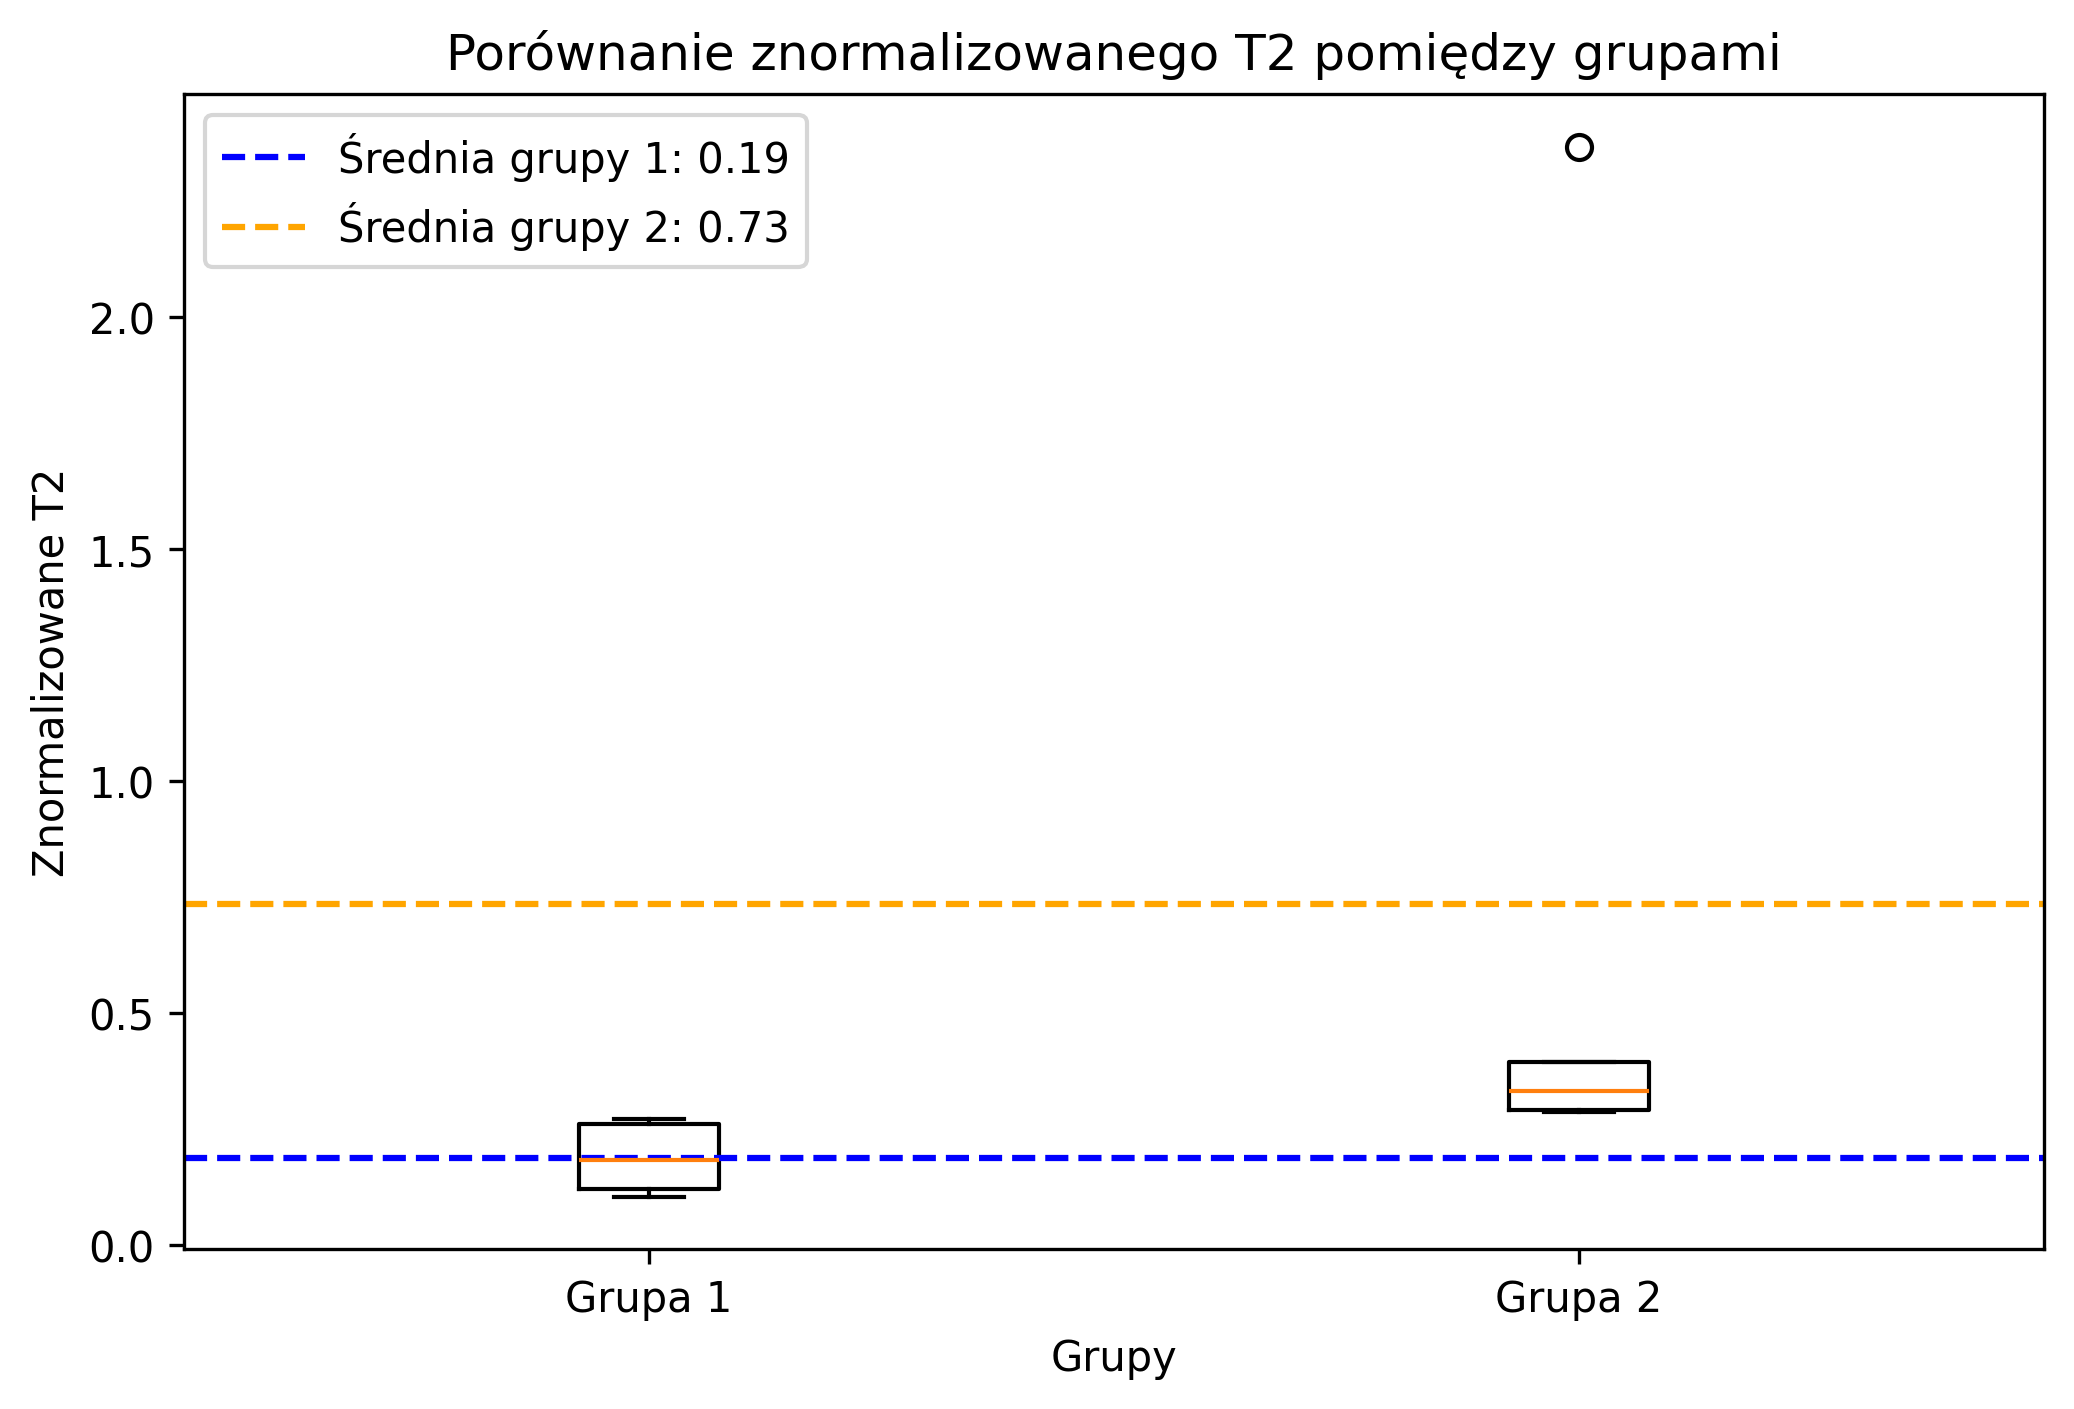
\includegraphics[width=0.8\linewidth]{diagramy/normalized_time_comparison}
    \caption{Wykres pudełkowy wyników obu grup}
    \label{fig:results_stats}
\end{figure}

Na Rysunku~\ref{fig:results_stats} przedstawiono wykres pudełkowy podsumowujący
pozyskane próbki.
Tabela~\ref{tab:wyniki_statystyka} przedstawia podstawowe wartości statystyczne.
Średnia grupy 2 jest o 74\% większa niż grupy 1.

\begin{table}[h]
    \centering
    \begin{tabular}{l|l|l|l|l|l}
        Grupa & Odchylenie standardowe & Średnia & Mediana & 25.\@ percentyl & 75.\@ percentyl \\ \hline \hline
        1 & 0.068 & 0.19 & 0.18 & 0.12 & 0.26 \\
        2 & 0.044 & 0.33 & 0.31 & 0.29 & 0.35 \\
    \end{tabular}
    \caption{\label{tab:wyniki_statystyka}Odchylenie standardowe, średnia, mediana, 25-ty i 75-ty percentyl w badanych grupach}
\end{table}

\section{Testowanie \(H_{0}\) t testem Welcha}

Test przeprowadzono przekazując zmierzone wartości \(T_{1}(i)\) i \(T_{2}(i)\),
następnie określając znormalizowaną wartość \((T_2^{norm}(i)\)otrzymując dwa
zbiory odpowiednie grupom.
Do funkcji przeprowadzającej t test \texttt{ttest\_ind} z biblioteki
\texttt{scipy.stats}~\cite{gonccalves2023effect} wprowadzono oba zbiory i
przetestowano, korzystając z parametrów uruchamiających t~test Welcha.

\lstinputlisting[language=Python,
    caption=\lstname,
    label={lst:ttest}]{ttest.py}

Wynikiem skryptu jest wydruk na standardowe wyjście przedstawione na Listingu~\ref{lst:ttest_output}.

\begin{lstlisting}[caption={Standardowe wyjście skryptu \texttt{ttest.py}},
    label={lst:ttest_output}]
First group seconds normalized: [0.2604834731129748, 0.10465116279069768, 0.27124773960216997, 0.1205298013245033, 0.18421052631578946]
Second group seconds normalized: [0.2860659773510586, 0.291970802919708, 0.3321764997521071, 0.3957131079967024]
First group mean: 0.18822454062922706
Second group mean: 0.32648159700489404
t value: -3.2386981867032234
p value: 0.01478208258587689
\end{lstlisting}

Dla potwierdzenia poprawności wprowadzonych danych można porównać wartości obu
grup \texttt{group normalized} z wydruku z danymi z Tabeli~\ref{tab:czas_norm}.
Wynikiem testu t Welcha jest wartość \(t = -3,23\) z \(p = 0,0148\).

Taka wartość \(t\) wskazuje, że wynik jest około 3,23-krotnie większy niż standardowy
błąd różnicy, co wskazuje na znaczną i statystycznie istotną różnicę pomiędzy
grupami.
Jednocześnie określa, że grupa rozwiązująca zadanie oparte o kod źródłowy o
niższym stopniu sprzężenia szybciej rozwiązała zadanie drugie.

\begin{figure}[h]
    \centering 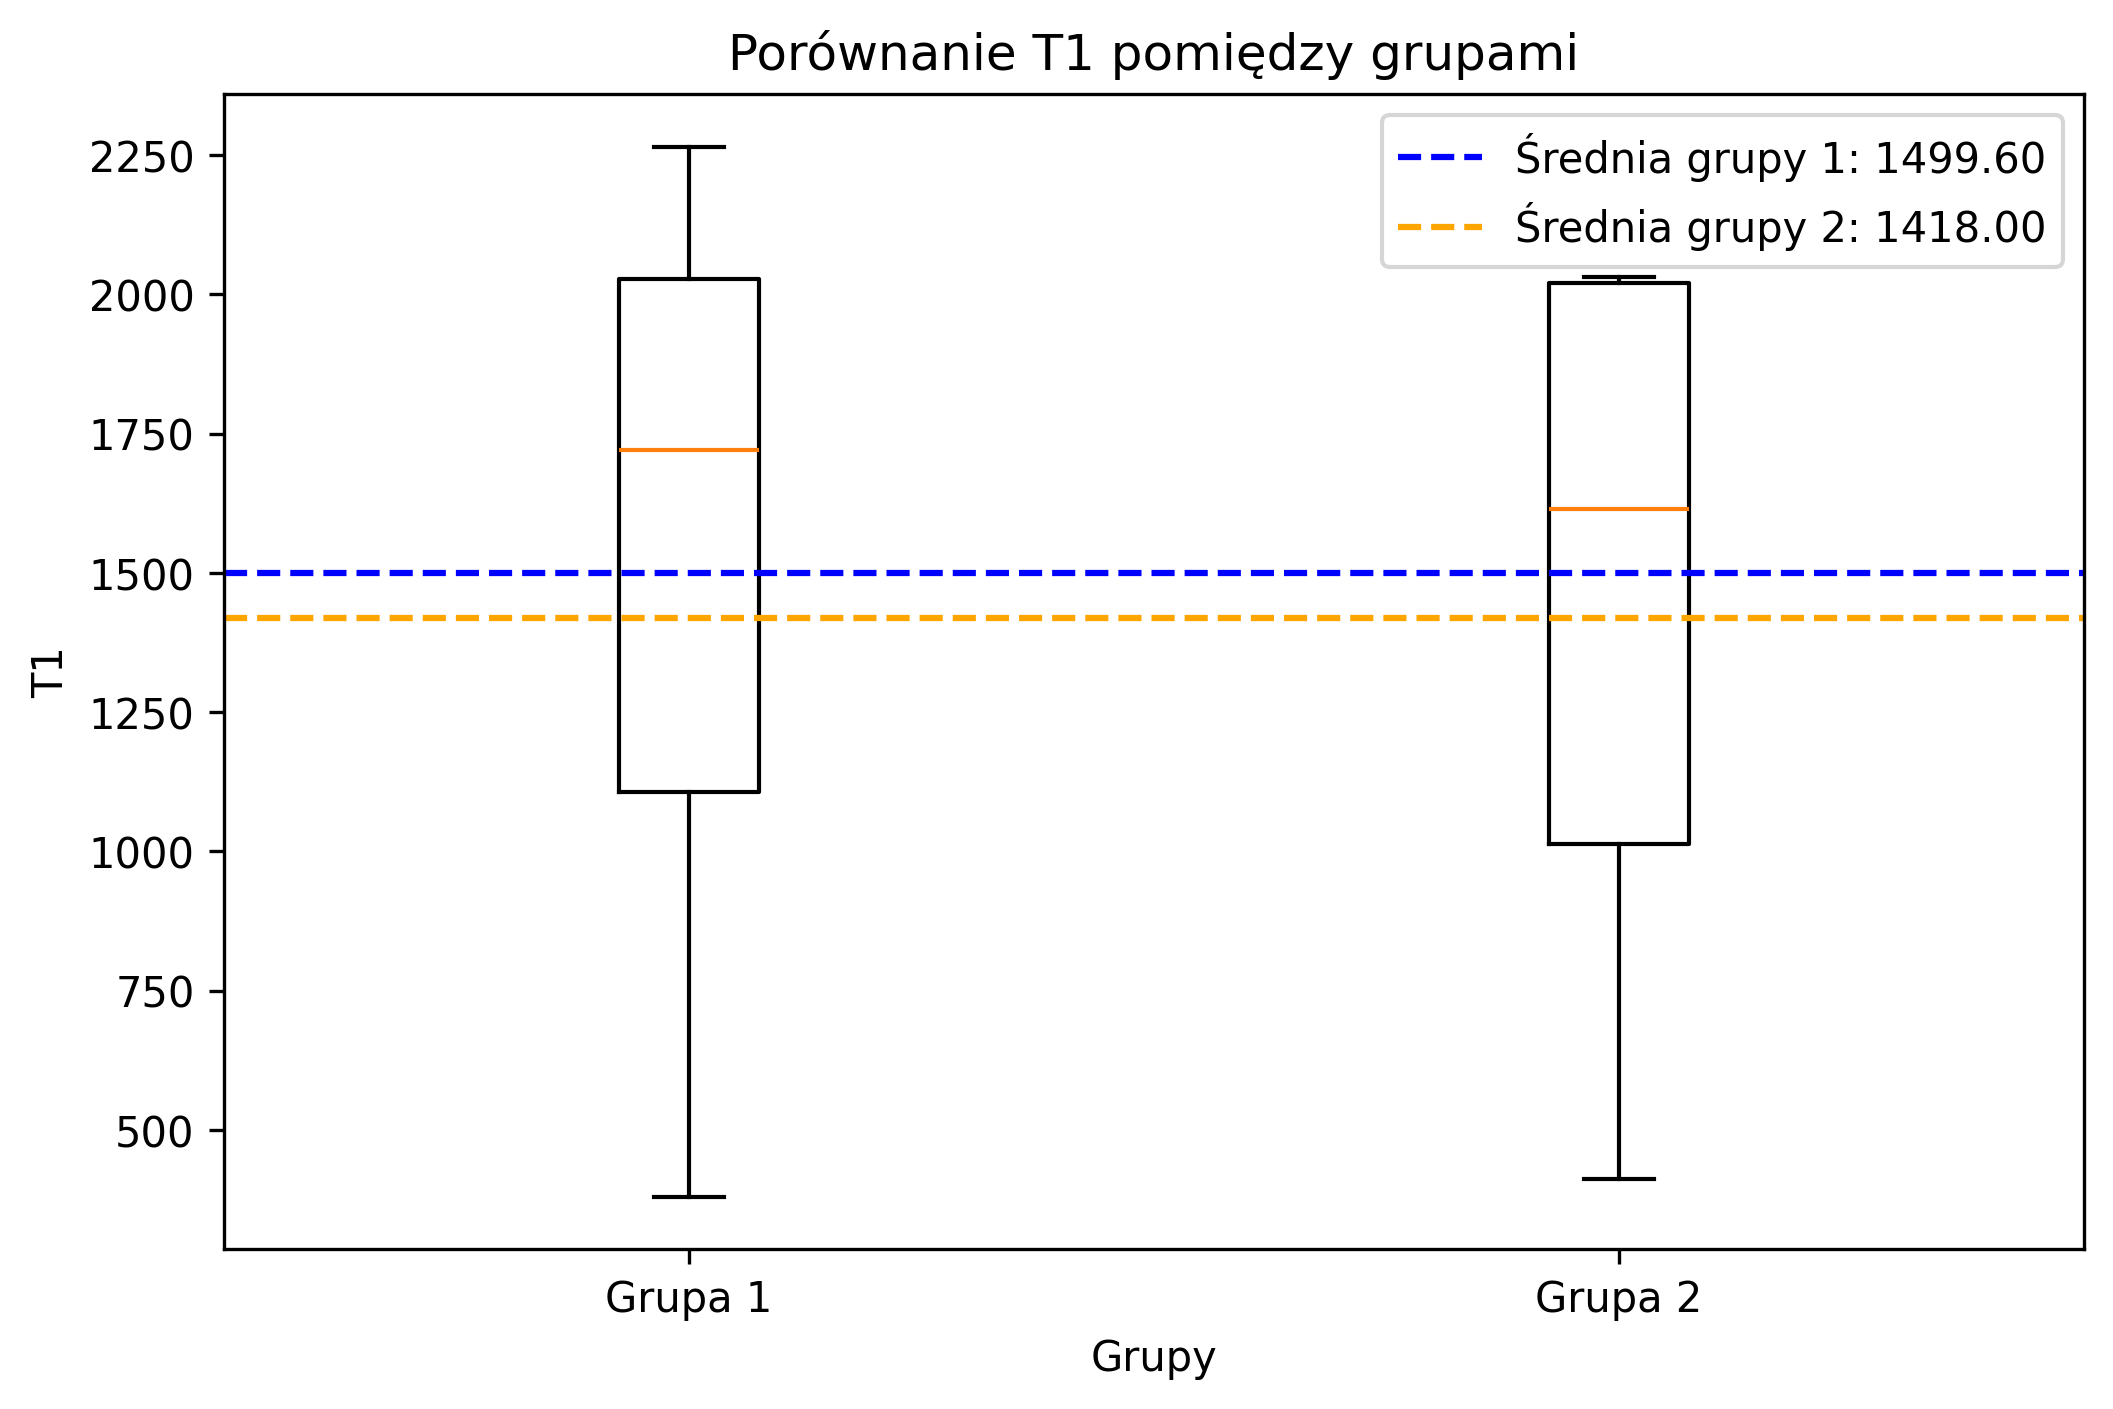
\includegraphics[width=0.7\linewidth]{diagramy/normalized_time_comparison_first}
    \caption{Wykres pudełkowy czasu \(T_{1}\) dla obu grup}
    \label{fig:results_first_status}
\end{figure}

Dodatkowo warto zbadać różnice w grupach pomiędzy czasem wykonywania zadania
kontrolnego --- określonego czasem \(T_{1}\).
Jeżeli różnica czasów jest statystycznie istotna w grupach, oznaczałoby to, że
stopień sprzężenia pomiędzy klasami ma wpływ na zadanie z pozoru niedotyczące
obszaru i należy odrzucić cały eksperyment ze względu na brak potwierdzenia
podstawowego założenia.
Wykres~\ref{fig:results_first_status} przedstawia różnice czasu w obu grupach.
Test t Welcha w tym przypadku daje wartości \(t = 0,15\) i \(p = 0.87\) co
wskazuje, że różnice są statystycznie nieistotne, zatem czas wykonania zadania
kontrolnego nie różni się statystycznie pomiędzy grupami eksperymentu.

\begin{table}[h]
    \centering
    \begin{tabular}{l|l|l|l|l|l}
        Grupa & odchylenie standardowe & średnia & mediana & 25 percentyl & 75 percentyl \\ \hline \hline
        1 & 681.32 & 1499.6 & 1720.0 & 1106.0 & 2027.0 \\
        2 & 669.07 & 1418.0 & 1615.0 & 1012.5 & 2020.5 \\
    \end{tabular}
    \caption{\label{tab:wyniki_zadanie_pierwszestatystyka}
    Odchylenie standardowe,\
        średnia, mediana, 25-ty i 75-ty percentyl dla czasu wykonania zadania \
        kontrolnego w badanych grupach}
\end{table}

Przy założeniu, że \(p < 0.05\) jest wymagane do odrzucenia hipotezy zerowej
\(H_{0}\), w świetle przeprowadzonego testu należy ją odrzucić, tym samym
dane uzyskane eksperymentalnie świadczą o statystycznie istotnej zależności
pomiędzy stopniem sprzężenia klasy i czasem wprowadzenia zmian w jej kodzie.

\section{Podsumowanie}

W toku eksperymentu pozyskano 10 próbek, z czego jedną należało odrzucić
ze względu na brak spełnienia założenia o zapoznaniu się z kodem źródłowym
podczas wykonywania zadania kontrolnego.

Uzyskane wyniki potwierdzają założenie, że czas wykonania zadania kontrolnego
w obu grupach nie różni się.
W związku z tym, nie ma podstaw do odrzucenia eksperymentu z powodu założenia,
że zadanie kontrolne jest wykonywane w obszarze wspólnym dla obu wariantów
programu.

Wartości \(T_{2}^{norm}\) są statystycznie różne dla obu grup, a ich średnia
różni się o \(74\%\).

W związku z tym eksperyment dostarczył wyników, które pozwalają na odrzucenie
hipotezy zerowej \(H_{0}\) i przyjęcie hipotezy \(H_{1}\), która głosi występowanie
statystycznie istotnej różnicy czasu wprowadzania zmian pomiędzy tożsamymi
programami o różnym stopniu sprzężenia.
Dodatkowo uzyskane dane pozwalają stwierdzić, że czas ten jest wyższy dla programów
o wyższym stopniu sprzężenia.

Z powyższych informacji można wyciągnąć wnioski co do zaprojektowania eksperymentu,
użytecznych heurystyk dla praktyków inżynierii oprogramowania, a także dalszych badań
w tym wąskim obszarze wpływu struktury programu obiektowego na koszty jego utrzymania.


\chapter{Wnioski}


    % Bibliografia - musi być
    % Bibliography - must exist
    \bibliografia

    % Strony końcowe - można zakomentować, jeśli zbędne
    % Additional pages - comment out if not needed
    
    % Wykaz symboli i skrótów - patrz opis w tekście przykładowym
    \acronymslist
    % Spis rysunków
    \listoffigures
    % Spis tabel
    \listoftables
    % Załączniki (plik appendices.tex)
    \easyappendices
\end{document}
%%%%%%%%%%%%%%%%%%%%%%%%%%%%%%%%%%%%%%%%%%%%%%%%%%%%%%%%%%%%%%%%%%%%%%%%%%%

